\section{Theorie}
\label{sec:Theorie}
\subsection{Der harmonische Oszillator}
Ein harmonischer Oszillator ist ein physikalisches System, welches eine Schwingung ausführt. Das einfachste Beispiel
hierfür ist eine Feder, an welcher eine Masse  $m$ um die Ruhelage $x_0$ oszilliert.
%Abbildung einfügen
Ein harmonischer Oszillator kann dabei über die Differentialgleichung
\begin{equation}
    \ddot{x}+\omega^2\cdot x=0 \label{eqn:harmOsz}
\end{equation}
definiert werden. Im mechanischen Fall ist dabei $x$ der Ort, $\ddot{x}$ die zweite Ableitung des Ortes nach der Zeit,
also die Beschleunigung und $\omega$ eine Konstante, welche weitere Informationen über das System, wie zum Beispiel die
Masse $m$, ergänzt. Zudem wird sich noch zeigen, dass $\omega$ die Frequenz der Schwingung beschreibt.
\\
Die Differentialgleichung kann bei der Feder aus dem zweiten Newton'schen Axiom
\begin{equation}
    F=m\cdot\ddot{x} \label{eqn:newton2}
\end{equation}
hergeleitet werden. Dafür wird das zweite Newton'sche Axiom der rücktreibenden Kraft der Feder gleichgesetzt. Die
Gleichheit der beiden Kräfte folgt aus dem Reaktionsprinzip. Die rücktreibende Kraft wird bei dem obrigen Beispiel
durch das Hook'sche Gesetz beschrieben
\begin{equation}
    F=-k\cdot x \label{eqn:hook}.
\end{equation}
Dabei ist $k$ die Federkonstante der Feder.
Gleichsetzen von \eqref{eqn:newton2} und \eqref{eqn:hook} liefert
\begin{equation}
    m\cdot\dddot{x}=-k\cdot x \Leftrightarrow \ddot{x}+\frac{k}{m}\cdot x=0 \label{eqn:dgl}.
\end{equation}
Gesucht ist nun die Funktion $x(t)$, die die Differentialgleichung löst. Ein geeigneter Ansatz für die Lösung ist:
\begin{align}
    x(t)&=A\cdot cos(\omega\cdot t)+B\cdot sin(\omega\cdot t) \\
    \ddot{x}(t)&=-\omega^2\cdot x(t)
    \label{eqn:ansatz}
\end{align}
$A$ und $B$ sind dabei Konstanten, die durch die Anfangsbedingungen bestimmt werden. Einsetzen des Ansatzes \eqref{eqn:ansatz}
in die Differentialgleichung \eqref{eqn:dgl} ergibt dann
\begin{equation}
    \biggl(A\cdot cos(\omega\cdot t)+B\cdot sin(\omega\cdot t)\biggr)\biggl(\frac{k}{m}-\omega^2\biggr)=0.
\end{equation}
Da der erste Faktor der Gleichung nicht für alle Zeiten $t=0$ sein kann, muss der zweite Faktor null ergeben
\begin{equation}
    \frac{k}{m}-\omega^2=0 \Leftrightarrow \frac{k}{m}=\omega^2 .
\end{equation}
Aus dem Ansatz \eqref{eqn:ansatz} wird nun auch ersichtlich, dass $\omega$ die Frequenz der Schwingung beschreibt. Dies erfolgt
unter anderem aus der Überlegung, dass das Produkt innerhalb des Sinus einheitenlos sein muss. Da die Zeit $t$ in Sekunden gegeben
ist, muss $\omega$ die Einheit $[\omega]=s^{-1}$ besitzen, also die Einheit einer Frequenz.
Die Schwingungsdauer $T$ des Pendels kann nun aus der Frequenz $\omega$ berechnet werden
\begin{equation}
  \label{eqn:omega}
    T=\frac{2\pi}{\omega}.
\end{equation}

\subsection{Das mathematische Pendel}
Auch ein mathematisches Pendel ist für kleine Auslenkungen näherungsweise ein harmonischer Oszillator. Das Pendel soll dabei eine
Punktmasse $m$ am Ende eines massenlosen Fadens sein, welcher eine konstante Länge $l$ hat und reibungsfrei hin und her schwingen kann.
Die Differentialgleichung folgt wieder aus dem Gleichsetzen von \eqref{eqn:newton2} und der rücktreibenden Kraft des Systems.
Diese ist nun aber:
\begin{equation}
    F_\text{rück}=-m\cdot g\cdot sin(\phi(t)) \label{eqn:pendelkraft}
\end{equation}
In \eqref{eqn:newton2} müssen wir jetzt noch die Beschleunigung $\ddot x$ an das Problem anpassen. Diese ist bei einem Pendel die tangentiale
Beschleunigung. Es gilt:
\begin{equation}
    \ddot x(t)=l\cdot \ddot{\phi}(t)
\end{equation}
Der Winkel $\phi(t)$ beschreibt dabei die Auslenkung des Pendels zum Zeitpunkt $t$. Gleichsetzen von \eqref{eqn:newton2} und
\eqref{eqn:pendelkraft} ergibt nun die Differentialgleichung
\begin{eqnarray}
    \ddot{\phi}(t)+\frac{g}{l}sin(\phi(t))=0.
\end{eqnarray}
Die Differentialgleichung ist auf Grund des Sinus jedoch nicht linear und deswegen weder analytisch lösbar, noch ein harmonischer Oszillator.
Um die Differentialgleichung trotzdem lösen zu können, betrachten wir die Taylorfunktion des Sinus
\begin{equation}
    sin(x)=\sum_{n=0}^\infty (-1)^n\frac{x^{2n+1}}{(2n+1)!}.
\end{equation}
Für $n=0$ ergibt sich die sogenannte Kleinwinkelnäherung
\begin{equation}
    sin(x)\approx x. \label{eqn:kleinwinkel}
\end{equation}
Durch diese wird zumindest für kleine Winkel $\phi$ eine lineare Differentialgleichung der Form \eqref{eqn:harmOsz} erlangt. Zwar entsteht bei der
Kleinwinkelnäherung ein Fehler, dieser ist für kleine Winkel jedoch so gering, dass wir die Näherung für die weiteren Berechnungen verwenden.
Dies bedeutet aber auch, dass im Folgenden nur noch von kleinen Auslenkungen des Pendels ausgegangen wird!
\\
Die Differentialgleichung lautet nun
\begin{equation}
    \ddot{\phi}(t)+\frac{g}{l}\phi(t)=0
\end{equation}
und wird durch den Ansatz \eqref{eqn:ansatz} gelöst. Die Frequenz ergibt sich dabei zu
\begin{equation}
    \omega=\sqrt{\frac{g}{l}}.
\end{equation}
Die Frequenz des Pendels ist also sowohl unabhängig von der Masse $m$, als auch von der Auslenkung, solange diese hinreichend klein ist.

\subsection{Das physikalische Pendel}
Anders als bei dem mathematischen Pendel ist die Masse des physikalischen Pendels nicht in einem Punkt am Ende eines massenlosen Fadens komprimiert.
Das Pendel hat nun auf der gesamten Länge eine Masse und kann beliebig geformt sein. Um die zusätzlichen Informationen in die Differentialgleichung
zu integrieren, wird die Größe des Trägheitsmoments $J$ eingeführt. Dieses ist definiert als
\begin{equation}
    J=\rho\int{\vec{r}^2\rho(\vec{r})dV}. \label{eqn:traegheit}
\end{equation}
Dabei ist $\rho$ die Dichte des Körpers an der jeweiligen Stelle.
\\
Die Differentialgleichung des Pendles wird dadurch zu
\begin{equation}
    \ddot{\phi}+\frac{mgl}{J}\phi=0.
\end{equation}
Die Frequenz ändert sich zu
\begin{equation}
    \omega=\frac{mgl}{J}.
\end{equation}

\subsection{Gekoppelte Pendel}
Werden zwei identische Pendel mit einer Feder gekoppelt, so schwingen diese nicht mehr unabhängig von einander, da die Pendel zusätzliche Kräfte auf
einander auswirken. Als zusätzlichen Größe fließt die Federkonstante $k$ in die Gleichung ein. Zudem sind nun zwei Längen für das System relevant, nämlich die
Länge der Pendel $L$ und der Abstand $l$, mit dem die Feder an den Pendeln befestigt ist.
\\
Es liegt nun ein System aus zwei Differentialgleichungen vor, die zudem miteinander gekoppelt sind:
\begin{align}
    J\ddot{\phi}_1&=-mgL\phi_1+kl^2(\phi_2-\phi_1)\\
    J\ddot{\phi}_2&=-mgL\phi_2+kl^2(\phi_2-\phi_1)
\end{align}
Das Differentialgleichungs-System wird im Folgenden nur für drei verschiedene Anfangsbedingungen gelöst, da nur diese für den Versuch relevant sind.
Die Anfangsbedingungen sind hierbei die Winkel $\alpha_1$ und $\alpha_2$, mit denen die Pendel zu Beginn ausgelenkt werden, und die Geschwindigkeiten
$v_1$ und $v_2$, die die Pendel zu Beginn erhalten. Für die drei relevanten Fälle gilt $v_1=v_2=0$.

\begin{enumerate}
    \item \textit{Gleichsinnige Schwingung: $\alpha_1=\alpha_2$} \\
        Bei einer gleichsinnigen Schwingung werden beide Pendel um den gleichen Winkel ausgelenkt. Die Pendel schwingen nun unabhängig von einander,
        so wie sie auch ohne eine Kopplung schwingen würden. Deswegen ist auch die Frequenz für mathematische Pendel analog zu jener, die wir für einzele
        mathematische Pendel her geleitet haben
        \begin{equation}
            \omega_{+}=\sqrt{\frac{g}{l}}.
        \end{equation}
        In Abbildung \ref{fig:gleichsinnig} ist die Amplitude der jeweiligen Schwingungen in Abhängigkeit von der Zeit aufgetragen. Wie gut zu erkennen ist, sind
        die Schwingungen identisch.
    \begin{figure}
        \centering
        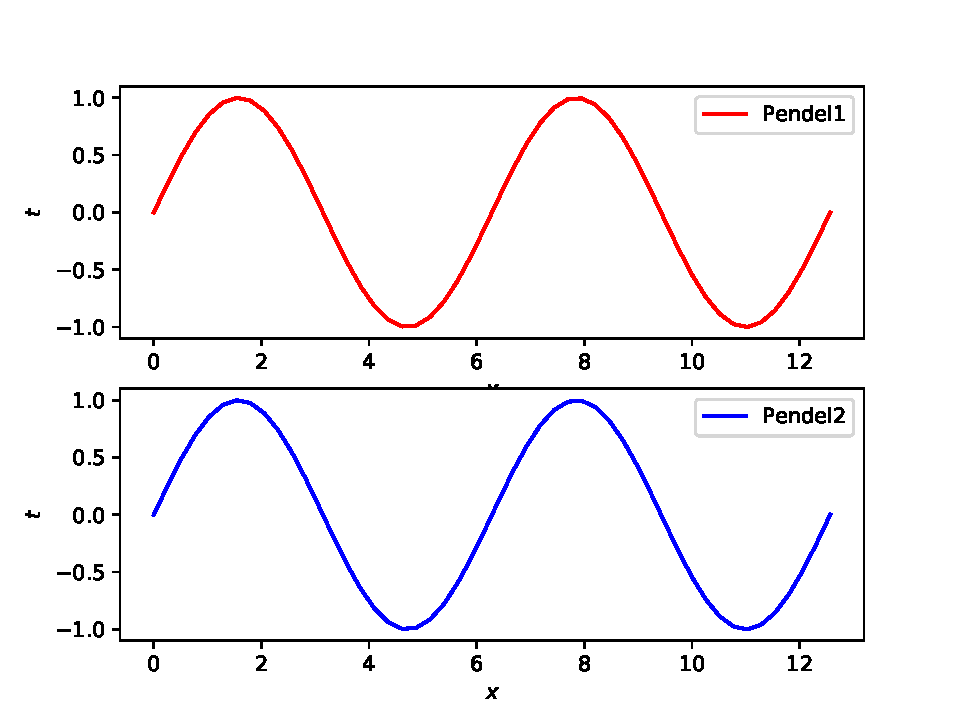
\includegraphics[scale = 0.7]{gleichsinnig.pdf}
        \caption{Amplituden in Abhängigkeit von t bei gleichsinniger Schwingung}
        \label{fig:gleichsinnig}
      \end{figure}
    \item \textit{Gegensinnige Schwingung: $\alpha_1=-\alpha_2$}\\
        Bei einer gegensinnigen Schwingung werden beide Pendel genau entgegengesetzt ausgelenkt. Der Betrag des Winkels ist also exakt gleich groß, das Vorzeichen
        ist jedoch genau entgegen gesetzt. Die Feder übt nun eine Kraft auf die Pendel aus, die abhängig von der Auslenkung der Pendel ist. Dadurch ergibt sich die
        Frequenz für mathematische Pendel zu
        \begin{equation}
            \omega_{-}=\sqrt{\frac{g}{l}+2\frac{kl^2}{mL^2}}.
        \end{equation}
        Die Frequenz hängt nun also auch noch von der Federkonstante $k$ ab. Wie in Abbildung \ref{fig:gegensinnig} zu erkennen, sind die Schwingungen der beiden
        Pendel um $\pi$ phasenverschoben. Ansonsten sind sie aber komplett identisch.
        \begin{figure}
            \centering
            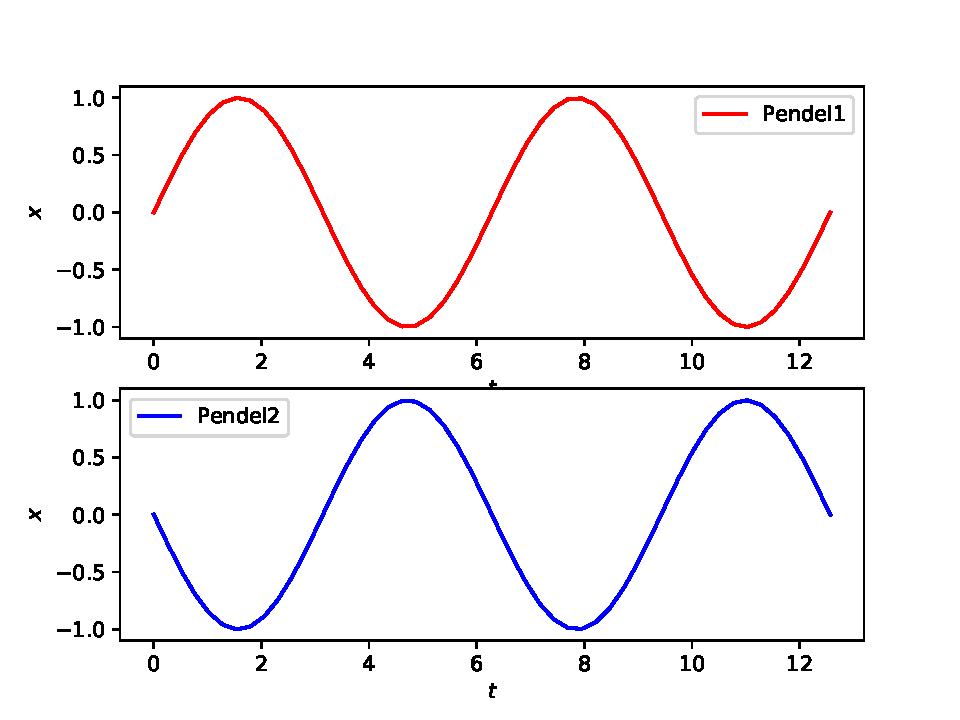
\includegraphics[scale = 0.7]{gegensinnig.pdf}
            \caption{Amplituden in Abhängigkeit von t bei gegensinniger Schwingung}
            \label{fig:gegensinnig}
        \end{figure}
    \item \textit{Gekoppelte Schwingung: $\alpha_1=0$, $\alpha_2\neq 0$}\\
        Bei einer gekoppelten Schwingung wird nur eines der beiden Pendel ausgelenkt. Das andere Pendel bleibt in der Ruhelage. Nun kommt es zu dem Phänomen der
        Schwebung. Das erste Pendel, welches ausgelenkt wird, überträgt bei seiner Schwingung seine Energie nach und nach an das zweite Pendel, welches sich
        zu Beginn in der Ruhelage befand. Dadurch fängt nun das zweite Pendel an zu schwingen. Hat das erste Pendel seine gesamte Energie an das zweite Pendel
        abgegeben, kommt es in der Ruhelage zum Stillstand. Das zweite Pendel, welches nun so schwingt wie das Erste zu Beginn, überträgt nun seine Energie wieder
        an das erste Pendel, bis sich der Vorgang abermals wiederholt. Die sogenannte Schwebungsfrequnz beschreibt nun die Zeitspanne zwischen dem Stillstand eines
        Pendels bis zum nächsten Stillstand des selben Pendels. Die Schwebungsfrequnz ist dabei gegeben durch
        \begin{equation}
            \omega_\text{S}=\omega_+ - \omega_-
        \end{equation}
        und die Schwebungsdauer ist gegeben durch
        \begin{equation}
            T_\text{S}=\frac{T_+\cdot T_-}{T_+-T_-}.
        \end{equation}
        In Abbildung \ref{fig:gekoppelt} sind zwei Schwebungen aufgetragen. Es ist zu erkennen, dass sich die Fuktion aus zwei überlagerten Schwingungen zusammensetzt.
        Die einhüllende Schwingung, also eine Funktion, die alle Maxima der gezeigten Funktion erfasst, charakterisiert hierbei die Schwebung als solche. Die Schwingung
        des Pendels selbst wir durch die darunter liegende Sinusfunktion beschrieben.
        \\
        Um die Kopplung zwischen den beiden Pendeln zu beschreiben, wird die Kopplungskonstante $K$ definiert
        \begin{equation}
          \label{eqn:kopplungskonstante}
            K=\frac{\omega_-^2-\omega_+^2}{\omega_-^2+\omega_+^2}=\frac{T_-^2-T_+^2}{T_-^2+T_+^2}.
        \end{equation}
        \begin{figure}
            \centering
            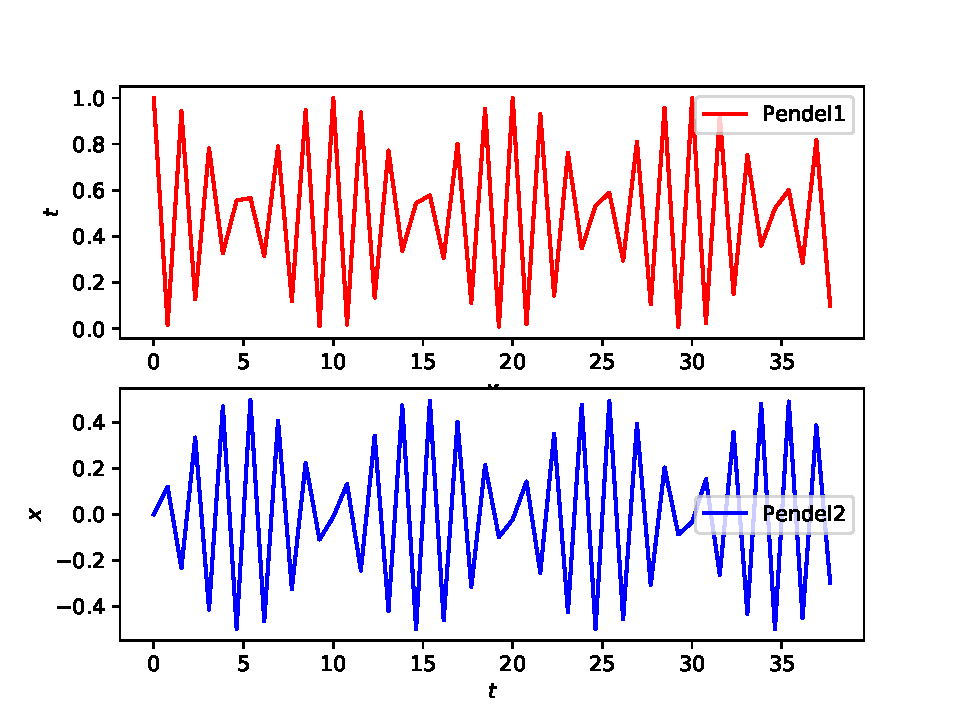
\includegraphics[scale = 0.7]{gekoppelt.pdf}
            \caption{Amplituden in Abhängigkeit von t bei gekoppelter Schwingung}
            \label{fig:gekoppelt}
        \end{figure}
\end{enumerate}
